\documentclass{exam}
\usepackage{../../commonheader}

%%% CHANGE THESE %%%%%%%%%%%%%%%%%%%%%%%%%%%%%%%%%%%%%%%%%%%%%%%%%%%%%%%%%%%%%%
\discnumber{2}
\title{\textsc{Mutable Data Structures and Data Abstractions}}
\date{February 15 to February 19, 2016}
%%%%%%%%%%%%%%%%%%%%%%%%%%%%%%%%%%%%%%%%%%%%%%%%%%%%%%%%%%%%%%%%%%%%%%%%%%%%%%%

\begin{document}
\maketitle
\rule{\textwidth}{0.15em}
\fontsize{12}{15}\selectfont

%%% INCLUDE TOPICS HERE %%%%%%%%%%%%%%%%%%%%%%%%%%%%%%%%%%%%%%%%%%%%%%%%%%%%%%%

\section{Lists}

\begin{questions}

%%% Question %%%

\begin{blocksection}
\question Draw box-and-pointer diagrams for the following.

\begin{lstlisting}
>>> a = [1, 2, 3]
>>> a
\end{lstlisting}
\begin{solution}[.25in]
\begin{lstlisting}
[1, 2, 3]
\end{lstlisting}
\end{solution}

\begin{lstlisting}
>>> a[2]
\end{lstlisting}
\begin{solution}[.25in]
3
\end{solution}

\begin{lstlisting}
>>> b = a
>>> a = a + [4, 5]
>>> a
\end{lstlisting}
\begin{solution}[.25in]
\begin{lstlisting}
[1, 2, 3, 4, 5]
\end{lstlisting}
\end{solution}

\begin{lstlisting}
>>> b
\end{lstlisting}
\begin{solution}[.25in]
\begin{lstlisting}
[1, 2, 3]
\end{lstlisting}
\end{solution}

\begin{lstlisting}
>>> c = a
>>> a = [4, 5]
>>> a
\end{lstlisting}
\begin{solution}[.25in]
\begin{lstlisting}
[4, 5]
\end{lstlisting}
\end{solution}

\begin{lstlisting}
>>> c
\end{lstlisting}
\begin{solution}[.25in]
\begin{lstlisting}
[1, 2, 3, 4, 5]
\end{lstlisting}
\end{solution}
\begin{solution}
\href{http://goo.gl/Gxe0qv}{Box and pointer diagram in Python Tutor.}
\end{solution}
\end{blocksection}

%%% Question %%%

\begin{blocksection}
\question Write a function that takes in a list \texttt{nums} and returns a
new list with only the primes from \texttt{nums}. Assume that
\texttt{is\char`_prime(n)} is defined. You may use a \texttt{while} loop, a
\texttt{for} loop, or a list comprehension.

\begin{lstlisting}
def all_primes(num):
\end{lstlisting}
\begin{solution}[2in]
\begin{lstlisting}
    result = []
    for i in nums:
        if is_prime(i):
            result = result + [i]
    return result

    List comprehension:
    return [x for x in nums if is_prime(x)]
\end{lstlisting}
\end{solution}
\end{blocksection}
\end{questions}

\section{Data Abstraction}
\begin{questions}

%%% Question %%%

\begin{blocksection}
\question The following is an \textbf{Abstract Data Type (ADT)} for elephants.
Each elephant keeps track of its name, age, and whether or not it can fly. Given
our provided constructor, fill out the selectors:

\begin{lstlisting}
def elephant(name, age, can_fly):
    """
    Takes in a string name, an int age, and a boolean can_fly.
    Constructs an elephant with these attributes.
    >>> dumbo = elephant("Dumbo", 10, True)
    >>> elephant_name(dumbo)
        "Dumbo"
    >>> elephant_age(dumbo)
        10
    >>> elephant_can_fly(dumbo)
        True
    """
    return [name, age, can_fly]
\end{lstlisting}

\begin{lstlisting}
def elephant_name(e):
\end{lstlisting}
\begin{solution}[1in]
\begin{lstlisting}
    return e[0]
\end{lstlisting}
\end{solution}

\begin{lstlisting}
def elephant_age(e):
\end{lstlisting}
\begin{solution}[1in]
\begin{lstlisting}
    return e[1]
\end{lstlisting}
\end{solution}

\begin{lstlisting}
def elephant_can_fly(e):
\end{lstlisting}
\begin{solution}[1in]
\begin{lstlisting}
    return e[2]
\end{lstlisting}
\end{solution}
\end{blocksection}

%%% Question %%%

\begin{blocksection}
\question This function returns the correct result, but there's something wrong
about its implementation. How do we fix it?

\begin{lstlisting}
def elephant_roster(elephants):
    """
    Takes in a list of elephants and returns a list of their names.
    """
    result = []
    for elephant in elephants:
        result = result + [elephant[0]]
    return result
\end{lstlisting}
\begin{solution}[1in]
\begin{lstlisting}[language=HTML]
elephant[0] is a Data Abstraction Violation (DAV).
We should use a selector instead.
\end{lstlisting}
\end{solution}

\end{blocksection}

%%% Question %%%

\begin{blocksection}
\question Fill out the following constructor for the given selectors.

\begin{lstlisting}
def elephant(name, age, can_fly):
\end{lstlisting}
\begin{solution}[1in]
\begin{lstlisting}
    return [[name, age], can_fly]
\end{lstlisting}
\end{solution}

\begin{lstlisting}
def elephant_name(e):
    return e[0][0]
\end{lstlisting}

\begin{lstlisting}
def elephant_age(e):
    return e[0][1]
\end{lstlisting}

\begin{lstlisting}
def elephant_can_fly(e):
    return e[1]
\end{lstlisting}

\end{blocksection}

%%% Question %%%

\begin{blocksection}
\question How can we write the fixed \texttt{elephant\char`_roster} function for
the constructors and selectors in the previous question?

\begin{solution}[2in]
No change is necessary to fix \texttt{elephant\char`_roster} since using the
\texttt{elephant} selectors ``protects'' the roster from constructor definition
changes.
\end{solution}

\end{blocksection}

\begin{blocksection}
\question \textbf{(Optional)} Fill out the following constructor for the given
selectors.

\begin{lstlisting}
def elephant(name, age, can_fly):
    """
    >>> chris = elephant("Chris Martin", 38, False)
    >>> elephant_name(chris)
        "Chris Martin"
    >>> elephant_age(chris)
        37
    >>> elephant_can_fly(chris)
        False
    """
    def select(command)
\end{lstlisting}
\begin{solution}[3in]
\begin{lstlisting}
        if command == "name":
            return name
        elif command == "age":
            return age
        elif command == "can_fly":
            return can_fly
        return "Breaking abstraction barrier!"
\end{lstlisting}
\end{solution}

\begin{lstlisting}
    return select
\end{lstlisting}

\begin{lstlisting}
def elephant_name(e):
    return e("name")
\end{lstlisting}

\begin{lstlisting}
def elephant_age(e):
    return e("age")
\end{lstlisting}

\begin{lstlisting}
def elephant_can_fly(e):
    return e("can_fly")
\end{lstlisting}

\end{blocksection}

\end{questions}

\newpage
\section{Trees}
\textbf{Things to remember}
\begin{lstlisting}
def tree(root, branches=[]): # ALWAYS OUTPUTS A TREE
    for branch in branches:
        assert is_tree(branch), 'branches must be trees'
    return [root] + list(branches)

def root(t): # ALWAYS OUTPUTS A NUMBER
    return t[0]

def branches(t): # ALWAYS OUTPUTS A LIST
    return t[1:]
\end{lstlisting}

\begin{questions}

%%% Question %%%

\begin{blocksection}
\question Draw the tree that is created by the following statement:

\begin{lstlisting}
tree(4,
    [tree(5, []),
     tree(2,
        [tree(2, []),
         tree(1, [])]),
     tree(1, []),
     tree(8,
        [tree(4, [])])])
\end{lstlisting}
\begin{solution}[4in]
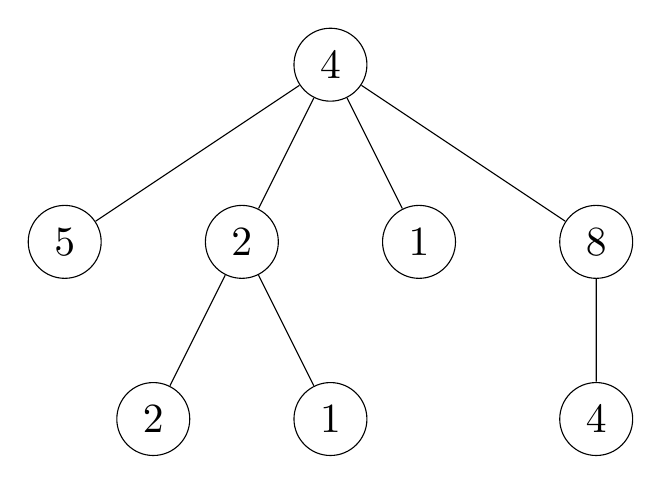
\begin{tikzpicture}[scale=1.5, transform shape]
    \node [circle, draw] (z){$4$}
        child {node [circle, draw] (a) {$5$}}
        child {node [circle, draw] (b) {$2$}
            child {node [circle, draw] (e) {$2$}}
            child {node [circle, draw] (f) {$1$}}
        }
        child {node [circle, draw] (c) {$1$}}
        child {node [circle, draw] (d) {$8$}
            child {node [circle, draw] (g) {$4$}}
        };
\end{tikzpicture}
\end{solution}

\end{blocksection}

\begin{blocksection}
\question Construct the following tree and save it to the variable \texttt{t}.

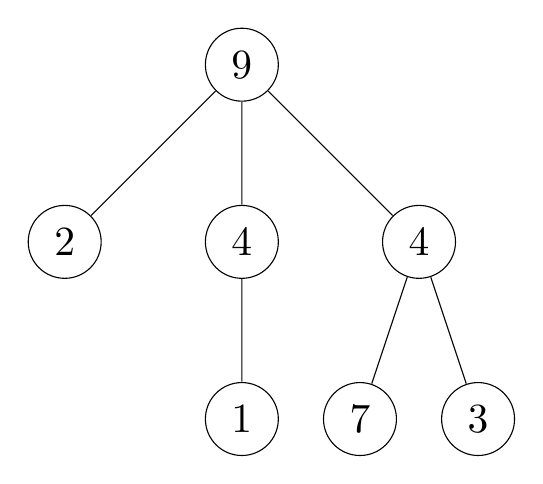
\begin{tikzpicture}[scale=1.5, transform shape]
\tikzstyle{level 2}=[sibling distance=10mm]
    \node [circle, draw] (z){$9$}
        child {node [circle, draw] (a) {$2$}}
        child {node [circle, draw] (d) {$4$}
            child {node [circle, draw] (g) {$1$}}
        }
        child {node [circle, draw] (b) {$4$}
            child {node [circle, draw] (e) {$7$}}
            child {node [circle, draw] (f) {$3$}}
        };
\end{tikzpicture}

\begin{solution}[4in]
\begin{lstlisting}
t = tree(9, [tree(2, []),
             tree(4, [tree(1, [])]),
             tree(4, [tree(7, []),
                      tree(3, [])])])
\end{lstlisting}
\end{solution}

\end{blocksection}

\begin{blocksection}
\question What would this output?

\begin{lstlisting}
>>> root(t)
\end{lstlisting}
\begin{solution}[.25in]
9
\end{solution}

\begin{lstlisting}
>>> branches(t)[2]
\end{lstlisting}
\begin{solution}[.25in]
\begin{lstlisting}
tree(4, [tree(7, []), tree(3, [])])
\end{lstlisting}
\end{solution}

\begin{lstlisting}
>>> branches(branches(t)[2])[0]
\end{lstlisting}
\begin{solution}[.25in]
\begin{lstlisting}
tree(7, [])
\end{lstlisting}
\end{solution}
\end{blocksection}

\begin{blocksection}
\question Write the Python expression to get the integer 2 from t.

\begin{solution}[0.25in]
\begin{lstlisting}
root(branches(t)[0])
\end{lstlisting}
\end{solution}

\end{blocksection}

\begin{blocksection}
\question Write the function \texttt{sum\char`_of\char`_nodes} which takes in a
tree and outputs the sum of all the elements in the tree.
\end{blocksection}

\begin{lstlisting}
def sum_of_nodes(t):
    """
    >>> t = Tree(...) # Tree from question 2.
    >>> sum_of_nodes(t) # 9 + 2 + 4 + 4 + 1 + 7 + 3 = 30
    30
    """
\end{lstlisting}
\begin{solution}[4in]
\begin{lstlisting}
    sum = 0
    for branch in branches(t):
        sum += sum_of_nodes(branch)
    sum += root(t)
    return sum

    Alternative solution:
    return root(t) +\
           sum([sum_of_nodes(b) for b in branches(t)])
\end{lstlisting}
\end{solution}

\end{questions}

%%%%%%%%%%%%%%%%%%%%%%%%%%%%%%%%%%%%%%%%%%%%%%%%%%%%%%%%%%%%%%%%%%%%%%%%%%%%%%%

\end{document}
